\documentclass[final]{beamer}

\usepackage[scale=1.24]{beamerposter} % Use the beamerposter package for laying out the poster
\usepackage{float}
\usepackage[export]{adjustbox}

\usetheme{confposter} % Use the confposter theme supplied with this template

\setbeamercolor{block title}{fg=ngreen,bg=white} % Colors of the block titles
\setbeamercolor{block body}{fg=black,bg=white} % Colors of the body of blocks
\setbeamercolor{block alerted title}{fg=white,bg=dblue!70} % Colors of the highlighted block titles
\setbeamercolor{block alerted body}{fg=black,bg=dblue!10} % Colors of the body of highlighted blocks
% Many more colors are available for use in beamerthemeconfposter.sty

%-----------------------------------------------------------
% Define the column widths and overall poster size
% To set effective sepwid, onecolwid and twocolwid values, first choose how many columns you want and how much separation you want between columns
% In this template, the separation width chosen is 0.024 of the paper width and a 4-column layout
% onecolwid should therefore be (1-(# of columns+1)*sepwid)/# of columns e.g. (1-(4+1)*0.024)/4 = 0.22
% Set twocolwid to be (2*onecolwid)+sepwid = 0.464
% Set threecolwid to be (3*onecolwid)+2*sepwid = 0.708

\newlength{\sepwid}
\newlength{\onecolwid}
\newlength{\twocolwid}
\newlength{\threecolwid}
\setlength{\paperwidth}{48in} % A0 width: 46.8in
\setlength{\paperheight}{36in} % A0 height: 33.1in
\setlength{\sepwid}{0.024\paperwidth} % Separation width (white space) between columns
\setlength{\onecolwid}{0.22\paperwidth} % Width of one column
\setlength{\twocolwid}{0.464\paperwidth} % Width of two columns
\setlength{\threecolwid}{0.708\paperwidth} % Width of three columns
\setlength{\topmargin}{-0.5in} % Reduce the top margin size
%-----------------------------------------------------------

\usepackage{graphicx}  % Required for including images

\usepackage{booktabs} % Top and bottom rules for tables

%----------------------------------------------------------------------------------------
%	TITLE SECTION 
%----------------------------------------------------------------------------------------

\title{Game of Life} % Poster title

\author{Devan Patel, Kyle Koceski, Daniel Fuentes} % Author(s)

\institute{CIS 4930: Concurrent Programming} % Institution(s)

%----------------------------------------------------------------------------------------

\begin{document}

\addtobeamertemplate{block end}{}{\vspace*{2ex}} % White space under blocks
\addtobeamertemplate{block alerted end}{}{\vspace*{2ex}} % White space under highlighted (alert) blocks

\setlength{\belowcaptionskip}{2ex} % White space under figures
\setlength\belowdisplayshortskip{2ex} % White space under equations

\begin{frame}[t] % The whole poster is enclosed in one beamer frame

\begin{columns}[t] % The whole poster consists of three major columns, the second of which is split into two columns twice - the [t] option aligns each column's content to the top

\begin{column}{\sepwid}\end{column} % Empty spacer column

\begin{column}{\onecolwid} % The first column

%----------------------------------------------------------------------------------------
%	INTRODUCTION
%----------------------------------------------------------------------------------------


\begin{block}{Introduction}
Jon Conway devised an algorithm to mimic cell automation in 1970, called the 'Game of Life'. Essentially, the game consists of a finite grid of cells that are either 'alive' or 'dead' and are dependent on the following rules:
\begin{itemize}
\item Any live cell with fewer than two live neighbours dies, as if caused by under-population.
\item Any live cell with two or three live neighbours lives on to the next generation.
\item Any live cell with more than three live neighbours dies, as if by overcrowding.
\item Any dead cell with exactly three live neighbours becomes a live cell, as if by reproduction.
\end{itemize}

\end{block}

%----------------------------------------------------------------------------------------
%	Objective
%----------------------------------------------------------------------------------------


\begin{block}{Objective}
	Our Game of Life implementation uses a server-client architecture, controlled and played on multiple clients. Iterations are computed on multiple clients; the server will constantly transmit the grid to clients after each iteration. When played, the server will distribute tasks of calculating iterations amongst the clients, and the calculations are returned to the server; it then merges the calculations, distributes the board and tasks to the clients again. Clients update grid size and initialialize living cells in order to play and then receive commands to calculate the next iteration. After these calculations are complete and sent to the server, client waits for future information.
\end{block}

%------------------------------------------------

\begin{figure}
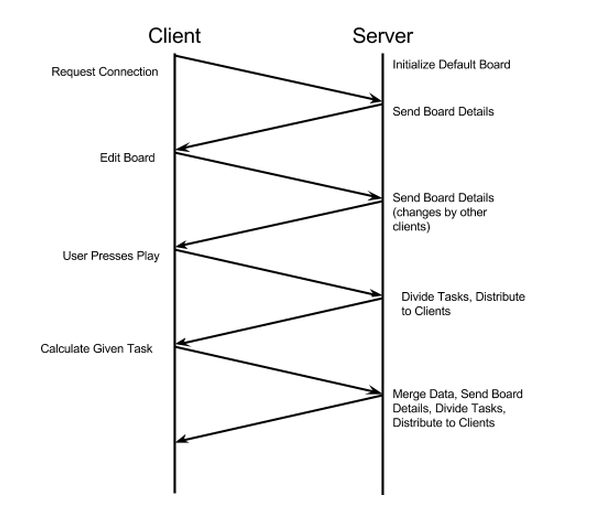
\includegraphics[width=0.8\linewidth]{client_server_architecture.jpg}
\caption{Client-server architecture}
\end{figure}

%----------------------------------------------------------------------------------------

\end{column} % End of the first column

\begin{column}{\sepwid}\end{column} % Empty spacer column

\begin{column}{\twocolwid} % Begin a column which is two columns wide (column 2)

\begin{columns}[t,totalwidth=\twocolwid] % Split up the two columns wide column

\begin{column}{\onecolwid}\vspace{-.6in} % The first column within column 2 (column 2.1)

%----------------------------------------------------------------------------------------
%	SCREENSHOT
%----------------------------------------------------------------------------------------

\begin{block}{}
\begin{figure}
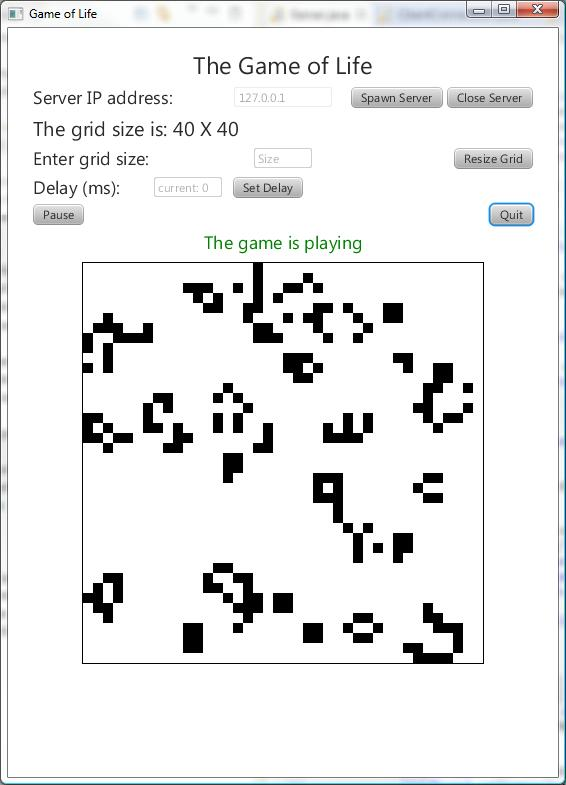
\includegraphics[width=.7\linewidth]{gol.jpg}
\caption{Game of Life in action!}
\end{figure}
\end{block}


\end{column} % End of column 2.1

\begin{column}{\onecolwid}\vspace{-.6in} % The second column within column 2 (column 2.2)
\begin{block}{}
\begin{figure}
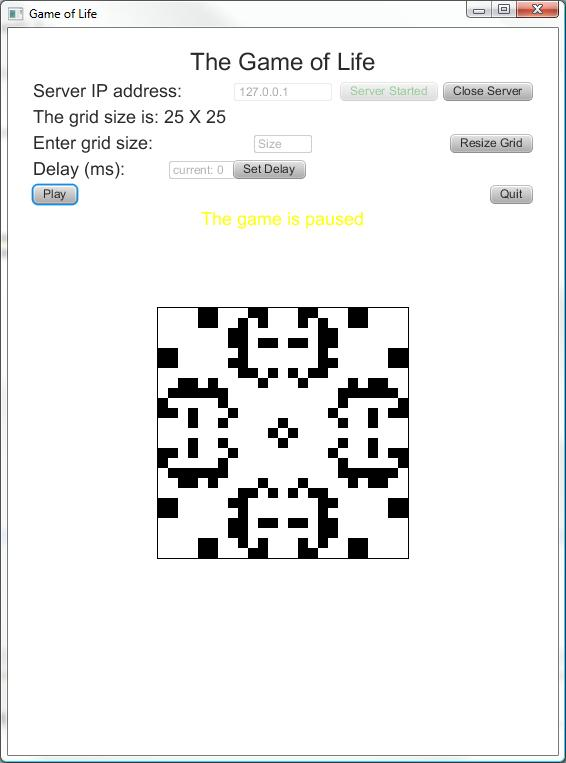
\includegraphics[width=.7\linewidth]{gol2.jpg}
\centering \caption{Unique patterns appear when ran long enough.}
\end{figure}
\end{block}

\end{column} % End of column 2.2

\end{columns} % End of the split of column 2 - any content after this will now take up 2 columns width

\begin{columns}[t,totalwidth=\twocolwid] % Split up the two columns wide column again

\begin{column}{\twocolwid} % The first column within column 2 (column 2.1)

%----------------------------------------------------------------------------------------
%	Results
%----------------------------------------------------------------------------------------

\begin{block}{Results}
The graphs below show when each calculation was either ran on the server or client and one or two clients with four lines representing one, two, four, or eight cores. 

\begin{figure}[!htb]
\minipage{0.48\textwidth}
  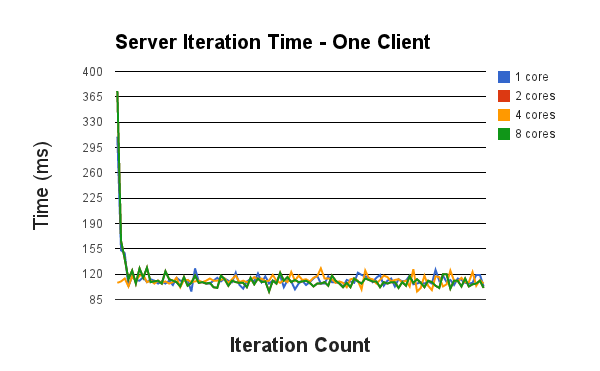
\includegraphics[width=\linewidth]{server-1.png}
\endminipage\hfill
\minipage{0.48\textwidth}
  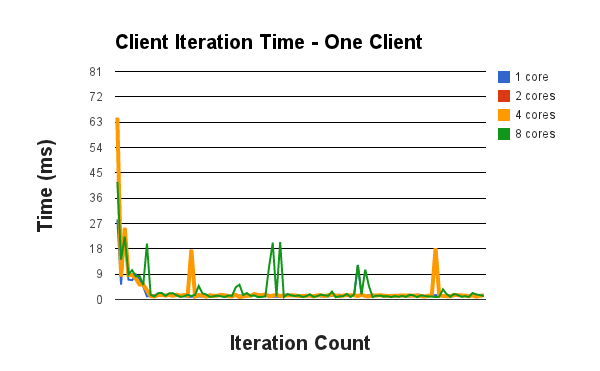
\includegraphics[width=\linewidth]{client-1.png}
\endminipage\hfill
\end{figure}

\begin{figure}[!htb]
\minipage{0.48\textwidth}
  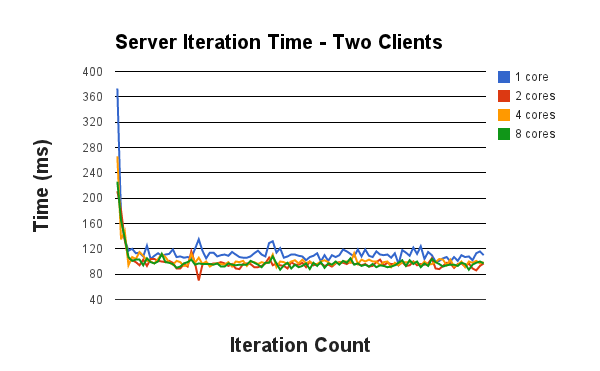
\includegraphics[width=\linewidth]{server-2.png}
\endminipage\hfill
\minipage{0.48\textwidth}
  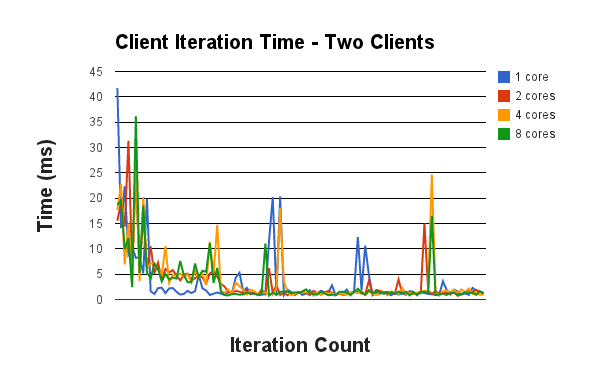
\includegraphics[width=\linewidth]{client-2.png}
\endminipage\hfill
\end{figure}

\end{block}

%----------------------------------------------------------------------------------------

\end{column} % End of column 2.1

\end{columns} % End of the split of column 2

\end{column} % End of the second column

\begin{column}{\sepwid}\end{column} % Empty spacer column

\begin{column}{\onecolwid} % The third column
%----------------------------------------------------------------------------------------
%	CONCURRENCY INVOLVED
%----------------------------------------------------------------------------------------

\begin{block}{Concurrency Involved}
\textbf{Server}:
\begin{itemize}
\item Synchronization on client list which is necessary to ensure a consistent view of the current clients before distributing tasks
\item Utilizing a lock for hash maps associating Connections to Tasks and Tasks to Returned Components
\item ''Barrier'' synchronization using Object.wait() and Object.notifyAll() to inform a thread when all clients have returned back partial calculation objects
\item Use of atomic references to hold cells for eliminating race conditions
\end{itemize}
\textbf{Client}:
\begin{itemize}
\item GUI thread and ClientConnection thread
\item ClientConnection uses JavaFX marshalling functions to receive information from Server and display the new grid to the user
\item Calculates the next iteration from the tasked partial components by distributing amongst threads (relatively equivalent to the number of available processors), sending back to server after threads complete
\end{itemize}
\end{block}

%----------------------------------------------------------------------------------------

%----------------------------------------------------------------------------------------
%	WHAT EACH MEMBER DID
%----------------------------------------------------------------------------------------
\begin{block}{Member Contributions}

\begin{itemize}
\item \textbf{Devan Patel} developed a concurrent algorithm determining neighboring cells, calculating the next iteration, and synchonously updating the grid.
\item\textbf{Kyle Koceski} managed the appropriate synchronization of multiple client threads and communication between clients and server.
\item\textbf{Daniel Fuentes} designed the graphical user interface that allowed clients to interact with the board, as well as displaying the board's current status, and the changes as the game progressed.
\end{itemize}
\end{block}

%----------------------------------------------------------------------------------------

\end{column} % End of the third column

\end{columns} % End of all the columns in the poster

\end{frame} % End of the enclosing frame

\end{document}